\documentclass[journal]{IEEEtran}
\usepackage[a5paper, margin=10mm, onecolumn]{geometry}
\usepackage[cmex10]{amsmath}
\usepackage{amssymb,amsfonts,amsthm}
\usepackage{gvv-book}
\usepackage{gvv}
\usepackage{hyperref}

\begin{document}


\title{2.4.20}
\author{EE25BTECH11025 - Ganachari Vishwambhar}
\maketitle

\textbf{Question}:\newline
Find the value of $\lambda$ such that the vectors $\vec{a}=2\vec{i}+\lambda\vec{j}+\vec{k}$ and $\vec{b}=\vec{i}+2\vec{j}+3\vec{k}$ are orthogonal.
\textbf{Solution: }\\
Given vectors are:
\begin{align}
    \vec{a}=\myvec{2\\\lambda\\1},
    \vec{b}=\myvec{1\\2\\3}
\end{align}

For two vectors to be orthogonal their dot product should be equal to zero which is equal to product of transpose column matrix $\vec{a}$ and column matrix $\vec{b}$:
\begin{align}
    \vec{a}^T\vec{b}=0\\
    \myvec{2&\lambda&1}\myvec{1\\2\\3}=0\\
    2+2\lambda+3=0\\
    \lambda=\brak{\frac{-5}{2}}
\end{align}

Therefore, the final vectors are:
\begin{align}
    \vec{a}=\myvec{2\\\brak{\frac{-5}{2}}\\1}\\
    \vec{b}=\myvec{1\\2\\3}
\end{align}

\begin{figure}[h!]
   \centering
   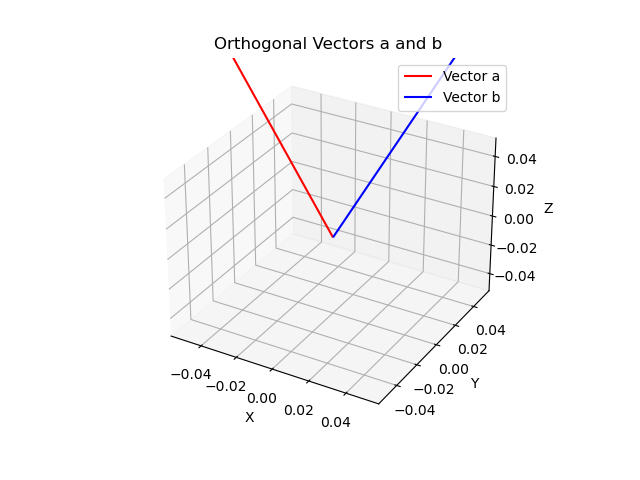
\includegraphics[width=0.7\linewidth]{figs/plot.png}
   \caption{Plot of orthogonal vectors $\vec{a}$ and $\vec{b}$}
   \label{}
\end{figure}
\end{document}  
